% =============================================================================
% CS224R Final Report — Conjecturer/Prover Self-Play for Countdown
% Build: pdflatex -> bibtex -> pdflatex x2   (or: python compile.py if present)
% =============================================================================
\documentclass{article}

\usepackage[preprint]{cs224r_2026}
\usepackage[utf8]{inputenc}
\usepackage[T1]{fontenc}
\usepackage{hyperref}
\usepackage{url}
\usepackage{booktabs}
\usepackage{amsfonts}
\usepackage{nicefrac}
\usepackage{microtype}
\usepackage{xcolor}
\usepackage{amsmath}
\usepackage{graphicx}
\usepackage{float}
\usepackage{enumitem}
\usepackage{listings}
\renewcommand{\lstlistingname}{Algorithm}

\lstset{
  basicstyle=\footnotesize\ttfamily,
  breaklines=true,
  frame=single,
  backgroundcolor=\color{gray!5},
  rulecolor=\color{gray!30},
  columns=fullflexible,
  keepspaces=true,
  captionpos=b
}

\title{When Can a Model Write Its Own Curriculum?\\
A Diagnostic Study of Joint Conjecturer/Prover RLOO for Countdown}

\author{%
  Nick Allen \\ \texttt{nallen21@stanford.edu} \\
  \And
  Finn St\"ablein \\ \texttt{finnst@stanford.edu} \\
}

\begin{document}
\maketitle

% =============================================================================
% ONE-PAGE EXTENDED ABSTRACT (2 pts) — standalone first page
% =============================================================================
\begin{center}\textbf{\large Extended Abstract}\end{center}

\noindent\textbf{Motivation and problem.}
Reinforcement learning from verifiable rewards (RLVR) -- where outputs are scored
by an automatic, typically rule-based verifier rather than a learned reward
model -- has driven recent reasoning gains, but it trains on a \emph{static} pool
of problems. We ask
whether a small model can instead \emph{generate its own curriculum}: a
conjecturer policy $C$ proposes problems and a prover policy $P$ solves them, so
that $C$ is rewarded for producing problems at $P$'s frontier of ability. We
study this on Countdown arithmetic, where a deterministic verifier scores both
$P$'s answers and (via a brute-force solver) whether $C$'s problems are even
solvable. Our central question is therefore not whether the joint approach outperforms
vanilla RLOO, but under what conditions two-policy self-play remains stable and
how it fails.

\noindent\textbf{Method and novelty.}
We implement the full default pipeline (SFT, IPO, RLOO) from scratch and build a
joint trainer on top of RLOO. Each step runs a nine-phase loop: sample $C$,
parse, solvability-filter, build prover prompts (mixed with fixed-dataset
problems for anchoring), sample $P$, score $P$ with the verifier and a length
penalty, compute $C$'s reward from the per-problem solve rate $\hat{p}$, and
RLOO-update both policies. To our knowledge this is the first application of a
conjecturer/prover loop to arithmetic reasoning with a \emph{rule-based} verifier
(prior conjecturer/prover work targets formal theorem proving). We contribute a
shaped difficulty-band reward $r_C=\max(0,\,1-2.5\,|\hat{p}-0.4|)$, a
solvability filter, and distributional anchoring via data mixing.

\noindent\textbf{Implementation and headline results.}
On 50 held-out problems ($k{=}16$ samples, fair eval at \texttt{max\_tokens}
${=}2048$), all RL methods raise pass@1 over the SFT baseline by a
statistically significant margin (paired bootstrap, 95\% CI excludes 0):
RLOO $0.244{\to}0.547$, Anchored-shaped $0.244{\to}0.515$, Conservative-binary $0.244{\to}0.345$.
At pass@16, \emph{no} method differs from SFT beyond noise (all CIs include 0).
The central finding is diagnostic: two-policy self-play is fragile in two
opposite directions. The Aggressive-binary configuration (high $C$ learning rate,
weak KL anchor) collapsed the curriculum to \emph{too-easy} problems (pass@16 fell
below SFT). The Anchored-shaped configuration (low $C$ learning rate, strong KL
anchor) failed in the opposite direction -- $C$ produced problems that were \emph{too hard}
($\hat{p}\approx0.05$ vs.\ target $0.4$) -- and, decisively, a
gradient-accumulation/solvability interaction silently \emph{starved} the
conjecturer of reward on 71\% of steps. We identify the bug, introduce a
pad-not-truncate fix. The corrected run (Anchored-shaped (fixed)) restores the curriculum mechanically -- the conjecturer is no longer starved and reaches the highest prover reward of any joint run -- yet still does not beat plain RLOO downstream, and weathers a transient mid-training collapse it recovers from.

\noindent\textbf{Discussion, limitations, conclusion.}
Our interpretation is that Anchored-shaped's gains are unlikely to be driven primarily by an
active curriculum -- which was live only $\sim$29\% of steps -- and are most
plausibly explained by ordinary RLOO on the fixed-dataset half of the prover's
training mix; a matched-sample RLOO control is needed to confirm this. Our limitations are real (n${=}50$, single
seed, 0.5B model, an eval-token-budget artifact we measured and corrected). The
principal lesson is methodological: stable conjecturer/prover self-play requires (i)
a dense reward signal that survives low solvability, (ii) a difficulty target
the conjecturer can actually hit, and (iii) instrumentation of curriculum health
(\texttt{valid\_rate}, $\hat{p}$) -- without which an apparently functional joint
run can be silently degenerate.

\newpage

% =============================================================================
% ABSTRACT (0.5 pts)
% =============================================================================
\begin{abstract}
We study whether a 0.5B language model can train itself by generating its own
problems, via a joint conjecturer/prover loop on Countdown arithmetic with a
rule-based verifier. After implementing SFT, IPO, and RLOO from scratch, we build
a nine-phase joint trainer with a shaped difficulty-band reward, a brute-force
solvability filter, and distributional anchoring. Across four configurations we
find that all RL methods significantly improve pass@1 over SFT but none
significantly change pass@16 (n${=}50$). More importantly, we map two opposite
failure modes of two-policy self-play -- collapse to too-easy problems under an
aggressive conjecturer update (high learning rate, weak KL anchor), and collapse
to too-hard problems plus a silent gradient-accumulation starvation under a
conservative one (low learning rate, strong KL anchor) -- and show that the
conjecturer received a reward signal on only
$\sim$29\% of steps. We diagnose the starvation bug and fix it; the corrected run restores the curriculum but still does not beat plain RLOO downstream. Our contribution is a rigorously documented negative result: a set of
necessary conditions, and the accompanying instrumentation, for stable curriculum self-play.
\end{abstract}

% =============================================================================
% 1 INTRODUCTION (2 pts)
% =============================================================================
\section{Introduction}
Reinforcement learning from verifiable rewards (RLVR) underlies much recent
progress in LLM reasoning~\cite{deepseekr1,gandhi2024sos}, but it optimizes a
policy against a \emph{fixed} set of training problems. As the policy improves,
many training problems become trivial and stop providing gradient, while the
hardest remain out of reach -- a static curriculum is rarely matched to the
model's moving frontier. A natural idea is to \emph{generate} the curriculum:
let one copy of the model (the \emph{conjecturer}, $C$) propose problems, and
reward it for proposing problems that a second copy (the \emph{prover}, $P$)
finds neither trivial nor impossible. We train both copies together by RLOO --
the \emph{joint} loop -- in contrast to vanilla RLOO, which trains a single policy
on a fixed problem set. Because Countdown is cheaply
verifiable -- and, crucially, problems are cheaply checkable for
\emph{solvability} by brute force -- it is an ideal testbed for this idea with a
rule-based reward rather than a learned one.

Conjecturer/prover self-play has been explored for \emph{formal} theorem
proving against a proof checker~\cite{dongma} and as multi-agent
co-evolution~\cite{subramaniam}, but not, to our knowledge, for arithmetic
reasoning with a rule-based verifier. We implement such a system and study it
empirically. Our guiding research questions are:
\begin{enumerate}[leftmargin=1.4em,itemsep=1pt]
  \item Can a jointly trained conjecturer/prover loop match or beat
  vanilla RLOO at lower sample cost on Countdown?
  \item When does two-policy self-play \emph{fail}, and what are the
  failure modes?
  \item Does the curriculum actually drive any observed gains, or
  do they come from the underlying RLOO and data mixing?
\end{enumerate}
In summary, the joint loop reaches pass@1 $0.515$ (Anchored-shaped) using roughly $6\times$
fewer update samples than vanilla RLOO ($0.547$), though no method improves
pass@16 beyond noise (RQ1); two-policy self-play collapses in opposite directions
 -- too-easy problems under an aggressive conjecturer update, too-hard
problems under a conservative one -- the latter compounded by a
gradient-accumulation interaction that starves the conjecturer entirely (RQ2);
and per-step instrumentation shows the curriculum was active on only $\sim$29\% of
steps, so Anchored-shaped's gains are most plausibly explained by ordinary RLOO on
the fixed-dataset half of the prover's training mix, rather than by the
conjecturer's curriculum (RQ3). We treat this negative result as our
central contribution.

% =============================================================================
% 2 RELATED WORK (2 pts)
% =============================================================================
\section{Related Work}
\textbf{RL from verifiable rewards.} DeepSeek-R1~\cite{deepseekr1} and
TinyZero~\cite{tinyzero} show that rule-based verifier rewards can elicit
strong reasoning, and the broader Countdown reasoning line~\cite{gandhi2024sos}
studies search and self-improvement in this domain -- but always on static
training data. We reuse that reward but make the \emph{data} adaptive.

\textbf{Preference and policy-gradient optimization.} We build on DPO/IPO
preference optimization~\cite{rafailov2023dpo,azar2023ipo} and REINFORCE
Leave-One-Out (RLOO)~\cite{ahmadian2024rloo}, which we implement directly; the
joint trainer reuses our RLOO update worker for both policies.

\textbf{Self-play and curricula.} Conjecturer/prover co-training has been applied
to formal proofs with a proof checker~\cite{dongma}; multi-agent
finetuning~\cite{subramaniam} trains several copies of a model on their own
self-generated data to preserve diverse reasoning and self-improve. Our
novelty is the combination of (i) a rule-based arithmetic verifier, (ii) a
brute-force \emph{solvability} filter that lets $C$'s reward be computed only on
genuinely solvable problems, and (iii) a shaped difficulty-band reward.

\textbf{Diversity collapse.} Kirk et al.~\cite{kirk2024understanding} document
that RLHF-style optimization can reduce output diversity. We observe an analogous
effect, together with its curriculum-side counterpart (collapse to systematically
easy or hard problems), and analyze it directly.

% =============================================================================
% 3 METHOD (5 pts)
% =============================================================================
\section{Method}
\subsection{Core pipeline}
All models are Qwen2.5-0.5B~\cite{qwen2025}. We warm-start with \textbf{SFT}
(completion-only cross-entropy), then study two alignment objectives.
\textbf{IPO}~\cite{azar2023ipo} minimizes
$\mathcal{L}_{\text{IPO}}=(h-\tfrac{1}{2\beta})^2$ where $h$ is the difference of
chosen/rejected log-ratios against a frozen SFT reference.
\textbf{RLOO}~\cite{ahmadian2024rloo} samples a group of $G$ responses per prompt
and uses the leave-one-out mean reward as the baseline; we apply a
clamped sequence-level importance weight to correct vLLM/HF logprob mismatch,
KL to the SFT reference, and gradient-norm clipping.

\subsection{Joint conjecturer/prover trainer (the extension)}
Two policies share the architecture and are both warm-started from SFT: the
conjecturer $C$ (problem generator) and the prover $P$ (solver). Each training
step executes the nine-phase loop shown in Figure~\ref{fig:method}.

\begin{figure}[h]
  \centering
  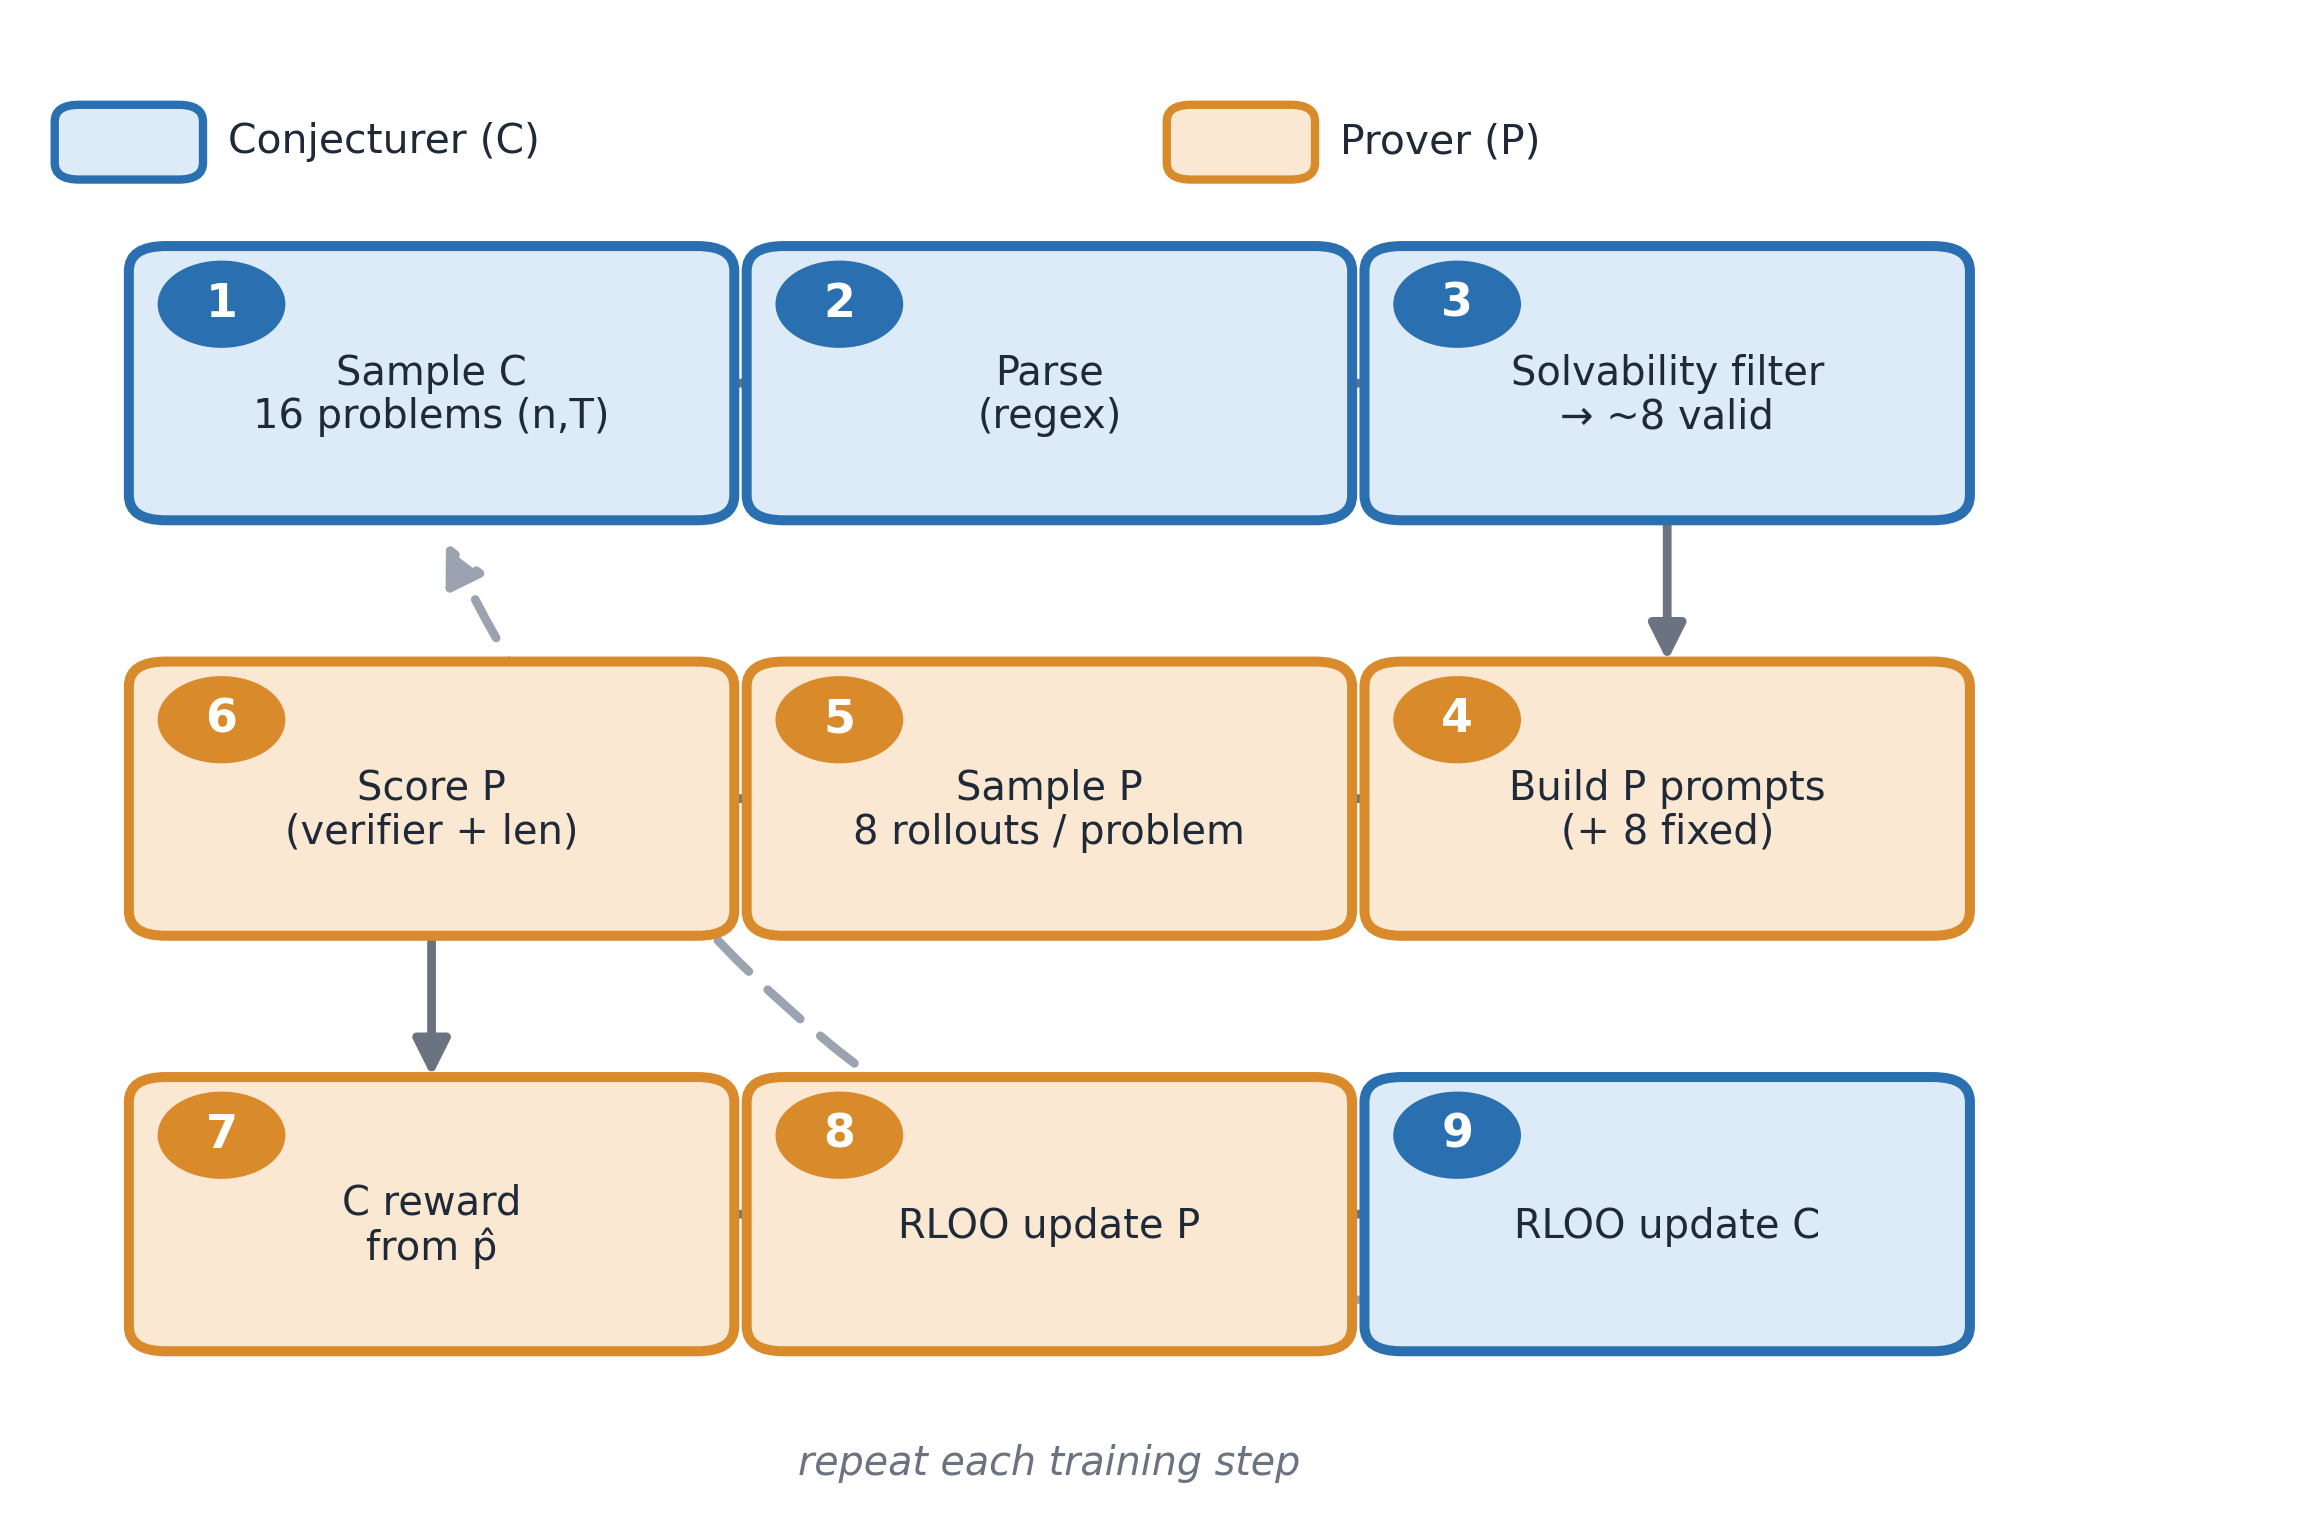
\includegraphics[width=0.92\linewidth]{figs/method_diagram.png}
  \caption{The nine-phase joint training step. Conjecturer phases (sample, parse,
  filter, update-$C$) in blue; prover phases (build prompts, sample, score,
  update-$P$) in orange; plus a shared reward-computation phase (compute
  $\hat{p}$, $r_C$). $C$'s reward is computed only on the solvable slice from
  $P$'s rollouts.}
  \label{fig:method}
\end{figure}


\noindent\textbf{Reward design.} $P$ receives the verifier score
($0$ malformed, $0.1$ well-formed but wrong, $1.0$ correct) minus a length
penalty $\alpha\cdot(\text{len}/\text{max\_len})$ that discourages excessively
long responses without hard truncation. $C$ receives a \emph{shaped tent} reward
$r_C=\max(0,1-2.5\,|\hat{p}-0.4|)$ peaking at solve-rate $\hat{p}=0.4$ and zero
outside $[0,0.8]$, replacing an earlier binary difficulty band. Only the
\emph{solvable} slice of problems can earn nonzero $r_C$, so the solvability
filter is essential.

\noindent\textbf{Anchoring and stability guards.} To keep $P$ from
over-specializing to $C$'s (possibly narrow) distribution, a fraction of each
prover batch is drawn from the fixed Countdown training set (50\% mix in Anchored-shaped). A
collapse guard rolls $C$ back to its last healthy checkpoint if its parseable
rate drops below a threshold. These were added in response to the failure modes
in Section~\ref{sec:results}.

\noindent\textbf{The starvation bug and its fix.}\label{para:starvation} The prover RLOO update requires
the \emph{total} batch (curriculum + fixed problems) to be divisible by the
gradient-accumulation factor $g$. The original code enforced this by truncating
the \emph{curriculum} count $n_{\text{valid}}$ down to a multiple of $g{=}8$.
When solvability is low (Section~\ref{sec:results}), $n_{\text{valid}}<8$ on most
steps, so it was truncated to \emph{zero} -- discarding every solvable problem and
leaving $C$'s reward vector all-zeros (zero policy gradient). The fix is to
\emph{pad} the total with fixed problems instead of truncating the curriculum, so
every solvable problem is kept. This is the key correction in our Anchored-shaped (fixed)
configuration.

% =============================================================================
% 4 EXPERIMENTAL SETUP (1 pt)
% =============================================================================
\section{Experimental Setup}
\noindent\textbf{Model/data.} Qwen2.5-0.5B-Base, SFT on the
\texttt{cog\_behav\_all\_strategies} Countdown corpus; verifier-based
prompts/solvability from \texttt{asingh15/countdown\_tasks\_3to4}.

\noindent\textbf{Baselines.} SFT (untrained on RL), and vanilla single-policy
RLOO at two checkpoints: step 80, its best-performing checkpoint by pass@1, and
step 30, an earlier checkpoint that shows the RLOO learning trajectory.

\noindent\textbf{Joint runs.} We name each configuration by its
conjecturer-update regime and its reward/anchoring scheme: Conservative-binary
and Aggressive-binary use a binary difficulty-band reward with no data mixing (a
conservative or aggressive conjecturer update, respectively), and Anchored-shaped
uses the shaped tent reward with 50\% fixed-data anchoring -- half of each prover
batch is drawn from the fixed Countdown set. See Table~\ref{tab:configs} for
hyperparameters.

\noindent\textbf{Evaluation.} 50 held-out problems, $k{=}16$ samples each, temp
$0.6$, top-$p$ $0.95$, top-$k$ $20$; pass@$k$ via the unbiased estimator of
Chen et al.~\cite{chen2021codex}. We report at \texttt{max\_tokens}${=}2048$ for
all directly compared models (see Section~\ref{sec:disc} for why this matters).

\noindent\textbf{Compute.} Single H100 via Modal; $\sim$3--4\,h per joint run.

\begin{table}[h]
\centering\small
\caption{Joint-run configurations. ``Mix'' = fraction of prover batch from the
fixed dataset; $c$-lr/$c$-KL are conjecturer-side. Anchored-shaped (fixed) is the corrected
configuration; we report its best preserved checkpoint (step 40), as the run collapsed at step 56.}
\label{tab:configs}
\begin{tabular}{lccccc}
\toprule
Run & $C$ reward & Mix & $c$-lr & $c$-KL & Steps \\
\midrule
Conservative-binary & binary band $[.05,.85]$ & 0\% & $5\!\times\!10^{-7}$ & 0.02 & 25 \\
Aggressive-binary & binary band $[.05,.75]$ & 0\% & $1\!\times\!10^{-5}$ & 0.001 & $\sim$30 \\
Anchored-shaped & shaped tent, peak $0.4$ & 50\% & $1\!\times\!10^{-6}$ & 0.02 & 100 \\
Anchored-shaped (fixed) & shaped tent (+ pad fix) & 50\% & $1\!\times\!10^{-6}$ & 0.02 & 100 \\
\bottomrule
\end{tabular}
\end{table}

% =============================================================================
% 5 RESULTS (6 pts)
% =============================================================================
\section{Results}
\label{sec:results}
\subsection{Quantitative evaluation}
Table~\ref{tab:passk} reports fair-eval pass@$k$; Table~\ref{tab:ci} reports
paired-bootstrap 95\% CIs (10k resamples over the 50 problems) for the change vs.\
SFT. Figure~\ref{fig:passk} visualizes the comparison.

\begin{table}[h]
\centering\small
\caption{Pass@$k$ on 50 held-out problems, $k{=}16$ samples,
\texttt{max\_tokens}${=}2048$.}
\label{tab:passk}
\begin{tabular}{lcccc}
\toprule
Model & pass@1 & pass@4 & pass@8 & pass@16 \\
\midrule
SFT baseline        & 0.244 & 0.534 & 0.669 & 0.760 \\
RLOO (step 30)      & 0.394 & 0.565 & 0.599 & 0.620 \\
RLOO (step 80, best)& \textbf{0.547} & 0.694 & 0.718 & 0.740 \\
Joint Conservative-binary (step 16)  & 0.345 & 0.651 & 0.748 & \textbf{0.800} \\
Joint Anchored-shaped (latest)   & 0.515 & 0.654 & 0.704 & 0.760 \\
Joint Anchored-shaped (fixed, step 40) & 0.455 & 0.633 & 0.666 & 0.680 \\
\bottomrule
\end{tabular}
\end{table}

\begin{table}[h]
\centering\small
\caption{Paired bootstrap (95\% CI) for the change in pass@$k$ relative to SFT.}
\label{tab:ci}
\begin{tabular}{lcc}
\toprule
Comparison & $\Delta$pass@1 [95\% CI] & $\Delta$pass@16 [95\% CI] \\
\midrule
RLOO 80 $-$ SFT & $+0.304$ $[+0.219,+0.391]^{*}$ & $-0.020$ $[-0.120,+0.080]$ \\
Joint Anchored-shaped $-$ SFT & $+0.271$ $[+0.176,+0.364]^{*}$ & $+0.000$ $[-0.100,+0.100]$ \\
Joint Conservative-binary $-$ SFT & $+0.101$ $[+0.044,+0.163]^{*}$ & $+0.040$ $[-0.040,+0.120]$ \\
Joint Anchored-shaped (fixed) $-$ SFT & $+0.211$ $[+0.134,+0.291]^{*}$ & $-0.080$ $[-0.180,+0.000]$ \\
\bottomrule
\end{tabular}\\[2pt]
\footnotesize $^{*}$ CI excludes 0 (significant). All pass@16 CIs include 0.
\end{table}

\begin{figure}[h]
  \centering
  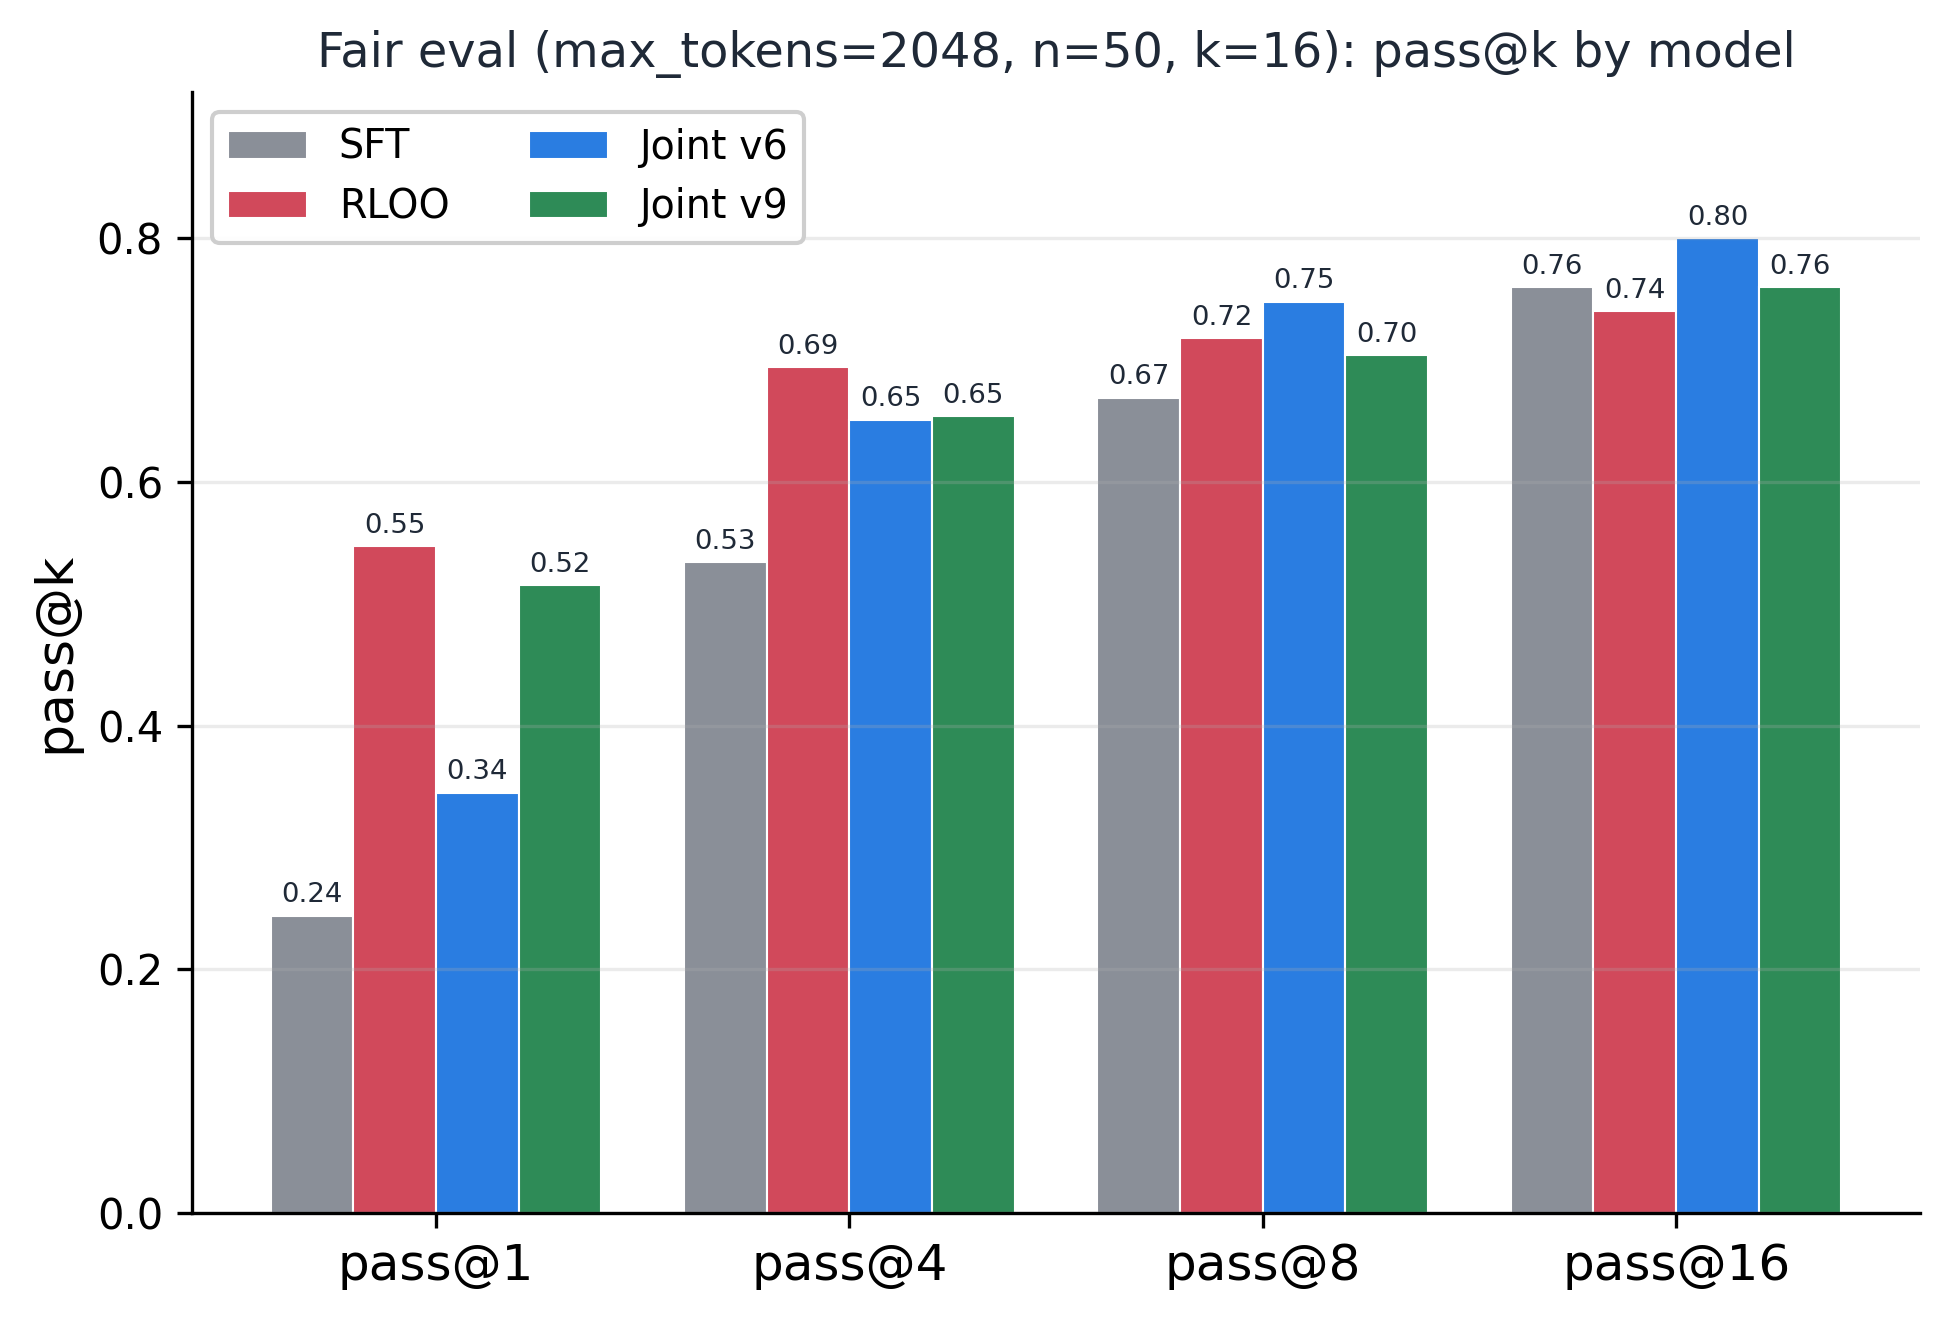
\includegraphics[width=0.7\linewidth]{figs/headline_passk_fair.png}
  \caption{Pass@$k$ at the fair \texttt{max\_tokens}${=}2048$ budget. RL methods
  separate from SFT at low $k$ and converge by $k{=}16$.}
  \label{fig:passk}
\end{figure}

\noindent\textbf{Principal findings.} (1) Every RL method significantly
improves pass@1 over SFT. (2) Anchored-shaped reaches pass@1 $0.515$ in $\sim$13k update
samples vs.\ RLOO's $0.547$ in $\sim$80k -- comparable accuracy at roughly
$6\times$ fewer samples (RQ1). (3) \emph{Crucially}, at pass@16 no method
differs from SFT beyond noise: the common claim that RLOO collapses output
diversity (pass@16 $0.740$ vs.\ $0.760$) is \emph{not} statistically supported at
n${=}50$. We therefore report pass@16 effects as suggestive, not conclusive.
The largest pass@16 drop, RLOO step~30 (0.620 vs.\ SFT 0.760), comes from an
under-trained intermediate checkpoint whose pass@16 is still climbing toward
step~80 (0.740); we therefore report CIs only for the deployable models (RLOO
step~80, Conservative-binary, Anchored-shaped), all of whose pass@16 differences from SFT fall within noise.

\subsection{Qualitative analysis: two failure modes}
\textbf{Aggressive-binary -- collapse to too-easy.} Updating the conjecturer
aggressively (high $C$ learning rate and batch size, weak KL anchor and entropy)
drove it toward ever-easier problems. During training, as the prover came to
solve almost everything the conjecturer produced, the per-problem solve rate $\hat{p}$
saturated near $1$, and the conjecturer's reward fell to zero ($c$-reward $\to 0$),
because its binary difficulty-band reward gives nothing once a problem falls
outside the target band -- here, problems the prover almost always solves. The prover,
trained on this collapsing distribution, in turn lost coverage on the held-out
set: its per-problem solve counts (out of 16 samples) became sharply bimodal --
19 of 50 problems solved $0$ times and 19 solved $\ge$12 times, with only 12 in
between -- the signature of mode collapse~\cite{kirk2024understanding}. Aggressive-binary is omitted from the fair-budget Table~\ref{tab:passk} because it
was evaluated only at the earlier \texttt{max\_tokens}${=}1024$ budget rather than
the $2048$ budget used for the other models. That budget systematically
under-counts pass@$k$ for any model whose reasoning exceeds it, the vanilla RLOO
baseline included (Sec.~\ref{sec:disc}).

\textbf{Anchored-shaped -- collapse to too-hard, plus silent starvation.} We instrumented
the loop and pulled per-step curriculum-health metrics from W\&B for the full
100-step Anchored-shaped run (Table~\ref{tab:health}). Two observations are notable. First, $C$'s
problems were systematically \emph{too hard}. Conditioning on the $\sim$29\% of
steps where $C$ actually produced solvable problems, the mean prover solve-rate
was $\hat{p}\lesssim0.17$ -- still well below the $0.4$ target (max ever $0.375$),
the opposite of Aggressive-binary. The all-steps mean of $0.05$ in Table~\ref{tab:health} is
additionally deflated because starved steps (no valid problems) log
$\hat{p}=0$ by construction. Second, and
decisively, the gradient-accumulation/solvability interaction
(Section~\ref{para:starvation}) drove the post-filter \texttt{valid\_rate} to
\emph{zero on 71\% of steps} (Figure~\ref{fig:curr_health}); \texttt{valid\_rate} only ever took the values
$\{0, 0.5\}=\{0/16, 8/16\}$ dictated by the $g{=}8$ truncation. Consequently
$C$'s reward was nonzero on only 29\% of steps. The conjecturer was
\emph{starved}: for most of training it received no gradient at all.

\begin{table}[h]
\centering\small
\caption{Anchored-shaped curriculum-health metrics over 100 steps (from W\&B). The
conjecturer received a reward signal on only $\sim$29\% of steps.}
\label{tab:health}
\begin{tabular}{lcccc}
\toprule
Metric & mean & max & \% steps $>0$ & note \\
\midrule
\texttt{c/parseable\_rate} & 0.92 & 1.00 & 100\% & $C$ stays well-formed \\
\texttt{c/valid\_rate}     & 0.145 & 0.50 & 29\% & 0 on 71\% of steps \\
\texttt{c/reward\_mean}    & 0.023 & 0.14 & 29\% & tiny even when nonzero \\
\texttt{c/p\_hat\_mean}    & 0.05 & 0.375 & 29\% & $\lesssim0.17$ on live steps; $\ll0.4$ \\
\texttt{c/frac\_too\_easy} & 0.01 & 0.25 & 9\% & opposite of Aggressive-binary \\
\bottomrule
\end{tabular}
\end{table}

\textbf{The answer to RQ3.} Because the curriculum was live on $\sim$29\% of
steps and miscalibrated when live, Anchored-shaped's gains are unlikely to be driven primarily
by an active curriculum and are most plausibly explained by ordinary RLOO on the
fixed-dataset half of the prover's training mix. The ``$6\times$ fewer samples'' comparison therefore conflates two factors, sample
count and the curriculum; disentangling them would require a matched-sample
control (RLOO trained on the same $\sim$13k samples), which we did not run. This
confound was apparent only from the per-step curriculum-health metrics. The
corrected configuration below sharpens the answer: even with the curriculum
demonstrably active, it does not beat RLOO, indicating the curriculum was not the
limiting factor on this task.

\textbf{Sample rollouts and conjectures.} A representative prover rollout
correctly reasons backward, e.g.\ for target 44 from $[26,4,2]$ it emits
\texttt{<answer> (26 - 4) * 2 </answer>}. The conjecturer emits well-formed
problems such as \texttt{<problem> numbers=[11, 39, 65], target=83 </problem>},
but most of them are not actually solvable.

\textbf{Generating solvable problems is itself hard.} To give the conjecturer a
stronger starting point, we also SFT'd it directly on (prompt, problem) pairs.
Even with a large ($\sim$400k-example) corpus it learned the output format almost
perfectly ($\approx$100\% parseable) yet produced mostly unsolvable problems --
only $\sim$20\% were solvable. The model captures the surface form of a Countdown problem without
internalizing the constraint that a solution must exist, a constraint that for
Countdown effectively requires solving the problem while generating it. At 0.5B
scale this appears to be a fundamental obstacle: proposing solvable,
appropriately-difficult instances may be harder than solving them, which bounds
how much a conjecturer can contribute to the curriculum for this task. It is also
the root of the too-hard collapse above -- the conjecturer's few solvable problems
skew hard -- and motivates the solvability-aware conjecturer objective we note as
future work.

\textbf{Corrected configuration: Anchored-shaped (fixed).} With the pad-not-truncate
fix every solvable problem is retained, so $C$ receives a reward signal on every
step that yields a solvable problem. This restores the curriculum
\emph{mechanically}: \texttt{c/valid\_rate} stays strictly positive throughout (vs.\
zero on 71\% of Anchored-shaped's steps), the conjecturer feeds $\sim$5--8 valid
problems to the prover each step, \texttt{c/p\_hat\_mean} rises through the $0.4$
target band (vs.\ Anchored-shaped's $\sim$0.05; Figure~\ref{fig:curr_health}), and
the prover's mean reward peaks at $0.65$ -- the highest of any joint run. Yet the corrected curriculum does
\emph{not} yield a better model. Its best preserved checkpoint (step 40) reaches
pass@1 $0.455$ -- above SFT ($+0.211$, 95\% CI excludes 0) but below both RLOO
($0.547$) and Anchored-shaped ($0.515$) -- and its pass@16 ($0.680$) is the lowest
in Table~\ref{tab:passk}, a diversity loss relative to SFT. The run also underwent
a \emph{transient} collapse around step 56 -- prover reward and $\hat{p}$ fell to
near zero for $\sim$25 steps -- but recovered to its pre-collapse level by step 85
(Figure~\ref{fig:v10recovery}), plausibly pulled back by the fixed-data RLOO
anchor; we read this as a robustness property rather than a terminal failure. The
step-40 checkpoint we report predates this recovery and is under-trained at 40
steps versus RLOO's 80 and Anchored-shaped's 100, so its weaker scores are partly a
training-length effect we cannot fully separate from the curriculum. The fix thus
confirms the diagnosis -- the starvation was real and removable -- yet shows that
making the curriculum function does not, on its own, beat plain RLOO on this task.

\begin{figure}[h]
  \centering
  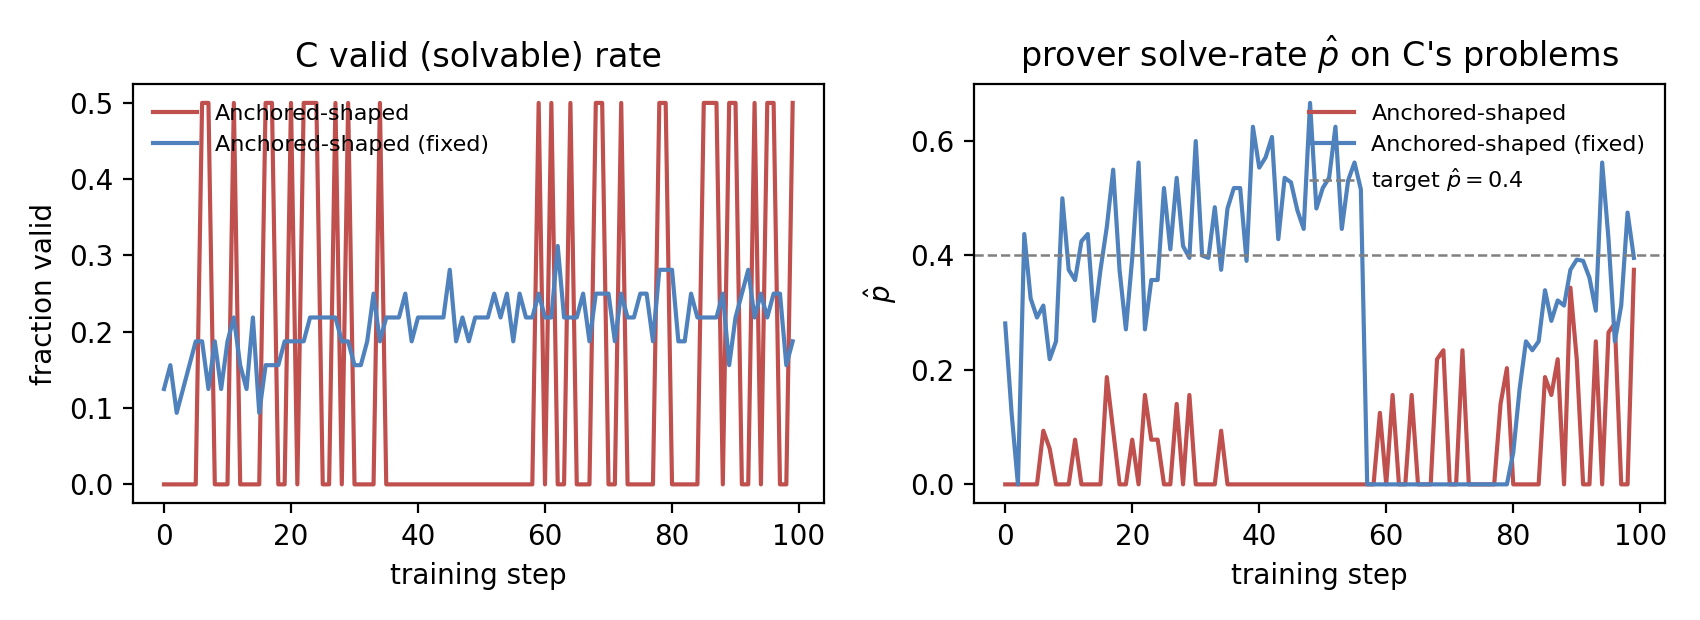
\includegraphics[width=0.95\linewidth]{figs/curriculum_health.png}
  \caption{Curriculum health, Anchored-shaped vs.\ Anchored-shaped (fixed).
  \emph{Left:} the fraction of $C$'s problems that are valid (parseable \&
  solvable) -- the unfixed run is starved to zero on most steps, the fixed run
  stays positive throughout. \emph{Right:} the prover solve-rate $\hat{p}$ on
  $C$'s problems -- the unfixed run sits near $0$ (too hard), the fixed run
  oscillates around the $0.4$ target.}
  \label{fig:curr_health}
\end{figure}

\begin{figure}[h]
  \centering
  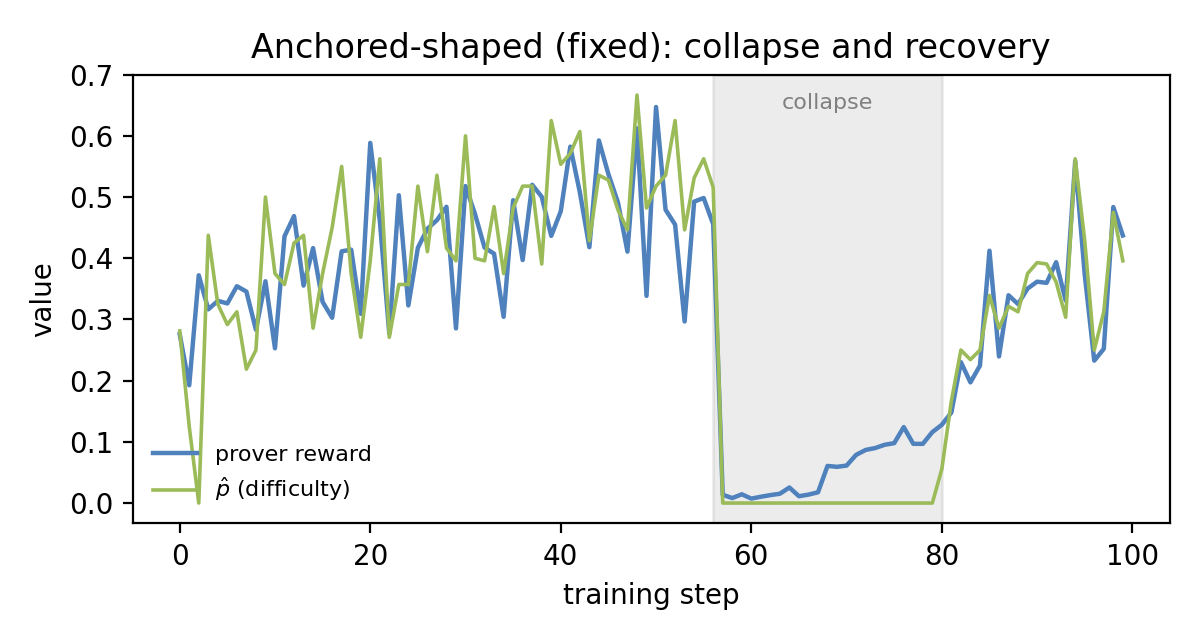
\includegraphics[width=0.62\linewidth]{figs/v10_collapse_recovery.png}
  \caption{Anchored-shaped (fixed) prover reward and difficulty $\hat{p}$ over
  training: a healthy phase peaking near step 50, a transient collapse (shaded,
  $\sim$steps 56--80), and recovery to the pre-collapse level by step 85.}
  \label{fig:v10recovery}
\end{figure}

% =============================================================================
% 6 DISCUSSION (0.5 pts)
% =============================================================================
\section{Discussion}
\label{sec:disc}
\noindent\textbf{Limitations.}
\begin{enumerate}[leftmargin=1.5em,itemsep=1pt,topsep=2pt]
  \item $n{=}50$ test problems, single seed -- paired-bootstrap CIs are wide and
  pass@16 differences are within noise.
  \item The 0.5B model makes collapse sharper than it might be at scale.
  \item We discovered an \emph{eval-token-budget artifact}: at
  \texttt{max\_tokens}${=}1024$, 269/271 Aggressive-binary failures hit the cap
  mid-reasoning before emitting \texttt{<answer>}, disproportionately penalizing
  more-verbose trained models; all compared numbers use 2048.
  \item The solver accepts non-integer intermediates, inheriting the verifier's
  true-division semantics.
\end{enumerate}

\noindent\textbf{Broader impacts.} Self-generated curricula can reduce the
human-annotation cost of RL training, but a model that writes its own problems can
amplify its own blind spots -- here, systematically too-hard problems -- when
curriculum health goes unmonitored; this makes our per-step health-logging
recommendation a safety-relevant practice rather than a convenience.

\noindent\textbf{Difficulties encountered.} The principal difficulty was that an
apparently successful joint run can be silently degenerate; only per-step
curriculum-health logging revealed the starvation.

% =============================================================================
% 7 CONCLUSION (0.5 pts)
% =============================================================================
\section{Conclusion}
A small model \emph{can} generate well-formed problems for itself, but turning
that into a useful curriculum is fragile. Two-policy self-play failed in two
opposite directions: collapse to too-easy problems under an aggressive conjecturer
update, and collapse to too-hard problems (with a silent starvation) under a
conservative one. The unfixed run's curriculum was active only $\sim$29\% of the
time; and when we fixed the starvation, the now-active curriculum still did not
beat plain RLOO and lost sample diversity -- though it did weather and recover from
a transient mid-training collapse, plausibly via the fixed-data anchor. The
curriculum was therefore not the limiting factor on this task. The principal contribution is a set of necessary
conditions for stable curriculum self-play: a reward dense enough to survive low
solvability, a difficulty target the conjecturer can actually reach, and
explicit curriculum-health monitoring. Future work: a solvability-aware $C$
objective, an adaptive difficulty band that tracks $P$'s skill, a clean
RLOO-at-matched-samples control to isolate the curriculum effect, and scaling to
3--7B models.

% =============================================================================
% 8 TEAM CONTRIBUTIONS (0.5 pts)
% =============================================================================
\section{Team Contributions}
The proposal listed three members; Nicolo dropped the course, leaving Nick Allen
and Finn St\"ablein. For the core implementation, Finn St\"ablein implemented the
supervised fine-tuning (SFT) stage and Nick Allen implemented the
preference-optimization (IPO) stage, and the two shared the RLOO implementation
and evaluation. The extension -- the joint conjecturer/prover trainer, its reward
design and solvability filter, the failure-mode diagnosis, and this report -- was
shared evenly between both members.

\bibliographystyle{plainnat}
\bibliography{reference}
\end{document}
